
\chapter{高可用和容错框架设计}


\section{故障分类和共性描述}

在章节\ref{failure_category}中,我们详细了解故障的分类。在本节中,我们将研究具体的故障情况,包括进程宕机、磁盘空间不足、网络分区等情况,分析故障的成因、表现和共性。

\subsection{进程宕机}

进程宕机,也称为进程崩溃或异常终止,是指一个正在运行的计算机进程由于遭遇某种无法处理的错误或异常情况,未能按照其正常的执行路径完成任务,而是以非预期的方式突然停止执行。

在进程宕机时,该进程提供的服务会立即中断或变得不可用。操作系统会检测到进程的异常终止,并回收该进程占用的系统资源,如内存、文件句柄、网络端口等。同时,操作系统或应用程序自身可能会记录宕机相关的错误信息。

导致进程宕机的原因分为程序内部错误和外部环境因素。

程序内部错误可以进一步划分为:
 
1. 非法内存访问: 尝试读取或写入程序无权访问的内存区域,例如野指针或空指针解引用、访问已释放的内存、数组越界等。

2. 未处理的异常: 程序逻辑中发生错误(如除以零),但没有相应的异常处理机制,来捕获和处理这些异常,导致程序终止。

3. 资源耗尽: 程序存在内存泄漏、文件句柄泄漏等问题,随着时间推移不断消耗系统资源,最终耗尽可用资源(如内存、文件描述符数量),导致操作系统强制终止进程,例如 Linux 的 OOM Killer 杀死内存超限的进程。

4. 多线程/并发问题: 复杂的竞争条件、死锁或线程同步错误。

外部环境因素可以进一步划分为:

1. 外部信号: 接收到操作系统或其他进程发送的强制终止信号,例如管理员执行 kill -9,发送 SIGKILL 信号,强制进程结束。

2. 外部软硬件故障:如内存条损坏导致进程读写数据错误、CPU 故障、磁盘 I/O 错误影响到程序加载或数据读写,或是进程依赖的动态链接库 (.so 文件) 丢失、损坏或版本不兼容。

3. 资源不足: 系统级别的资源不足,如物理内存或交换空间耗尽、硬盘空间不足,可能导致进程无法正常运行而被操作系统终止。

进程宕机在分布式系统中有明确的影响,包括:

1. 服务中断。该进程提供的服务、数据将无法处理和访问。

2. 数据丢失。如果在宕机时进程持有尚未持久化到稳定存储的关键内存状态,这些状态将会丢失,导致系统的状态不一致或数据资产的损失。

3. 造成级联影响。如果系统的其他组件和进程依赖这个进程,那么他们服务也会受到该进程宕机的影响。

\subsection{磁盘空间不足}

分布式系统中的磁盘空间不足故障,是指构成系统的某个或多个节点的本地存储设备(硬盘、SSD等)上的可用空间耗尽,无法再写入新的数据、日志文件、临时文件或执行需要磁盘空间的内部操作。

常见导致分布式节点磁盘空间不足的原因包括:

1. 写入速度和数据保留策略不恰当。例如在IoTDB中,数据写入速率可能非常高,在磁盘受限的情况下,如果保留时间被设置的很久,就会导致数据会不断累积,最终填满磁盘。

2. 日志文件的累积:在高写入负载下,WAL 文件会快速增长。在同步速度不足、WAL 归档或清理机制出现问题,WAL 文件可能会填满磁盘。此外,如果运行日志压缩和定期清理机制配置不当或失效,日志文件会无限增长并耗尽磁盘空间。

3. 临时缓存文件导致:系统在执行查询、排序、数据导入导出、内部维护任务时,可能会产生大量的临时文件。如果这些文件未能被及时清理,或者任务失败导致临时文件残留,会占用大量空间

4. 其他人为因素:本地快照如果未按计划清理或移动到长期存储、错误地将非数据库相关的大文件存放在数据库节点的数据盘上、磁盘挂载点配置错误或磁盘损坏导致部分空间不可用。

磁盘写满故障对于单节点和集群都会产生显著的影响。当磁盘空间不足时,节点会拒绝写入操作,同时内部的操作(如WAL、合并)等可能会失败,最后导致数据不一致、节点服务不稳定甚至宕机。对于集群来说,一个节点的磁盘满可能导致整个复制组的写入被阻塞或失败,从而降低整个集群的写入吞吐量和可用性。

\subsection{网络分区}

网络分区是指在一个分布式系统中,由于网络故障,部分节点之间无法正常通信,导致整个系统被分割成两个或多个相互隔离的子网络或“分区”。位于同一个分区内的节点可以相互通信,但无法与位于其他分区内的节点直接通信。

网络分区产生的原因包括:

1. 网络设备故障,例如路由器或交换机故障,或是单个服务器的网卡故障,导致所连接的节点之间的通信中断,形成分区。

2. 物理链路故障,连接服务器到交换机、或交换机与交换机之间的物理线缆可能因损坏(如被意外切断、老化、物理损伤)而导致通信中断。

3. 网络配置错误,防火墙规则配置错误、路由表错误、VLAN 配置问题、DNS 问题都可能会导致特定节点之间的通信中断。

4. 网络拥塞,当网络链路或网络设备的流量负载远超其处理能力时,数据包会被队列等待甚至被直接丢弃。持续严重的丢包和高延迟会导致分布式系统中的节点通信超时而被认为“失联”。

5. 恶意攻击,恶意攻击可能通过拒绝服务攻击 (DoS/DDoS)等方式瘫痪部分网络链路或节点,制造网络分区。

网络分区可能会造成严重的后果,包括:

1. 服务的中断和性能的下降。如果分区导致没有一个分区包含足够多的节点来维持核心服务的运行,整个分布式系统可能会变得不可用。即使部分服务仍然可用,由于集群规模缩小、数据副本不可用或需要切换到备用节点,整体吞吐量和延迟可能会显著下降。

2. 脑裂问题。发生分区时,两个或多个分区都错误地认为自己是合法的系统领导者身份,并独立地进行关键操作(如写入、资源分配、领导者决策)。这可能导致数据覆盖、数据损坏、资源重复分配等后果。

3. 提高协调难度。集群范围内的状态更新(如新的配置、拓扑变化、负载信息)无法跨越分区传播。这使得不同分区的节点对整个系统的视图变得陈旧和不一致,增加分区恢复后的协调难度。如果数据复制机制是异步的,分区会阻碍数据同步,导致不同副本之间的数据延迟增加,增加合并和冲突解决的难度。

网络分区还可以进一步划分为对称网络分区和非对称网络分区。

对称网络分区是网络分区的一种典型形式。它指的是网络故障导致节点间的通信断裂是双向的。也就是说,如果节点 A 无法发送消息到达节点 B,那么节点 B 也同样无法发送消息到达节点 A。通信的中断是相互的、对称的。

非对称网络分区指的是某些数据节点节点能够向其他节点发送消息,但是无法接收来自这些节点的消息,或者反过来,接收消息正常但发送消息受阻。

这种单向或双向但方向不同的通信故障,与传统的对称网络分区有着本质的区别。由于其特殊性,IoTDB内部需要对非对称网络分区有针对性的处置。

\begin{figure}
  \centering
  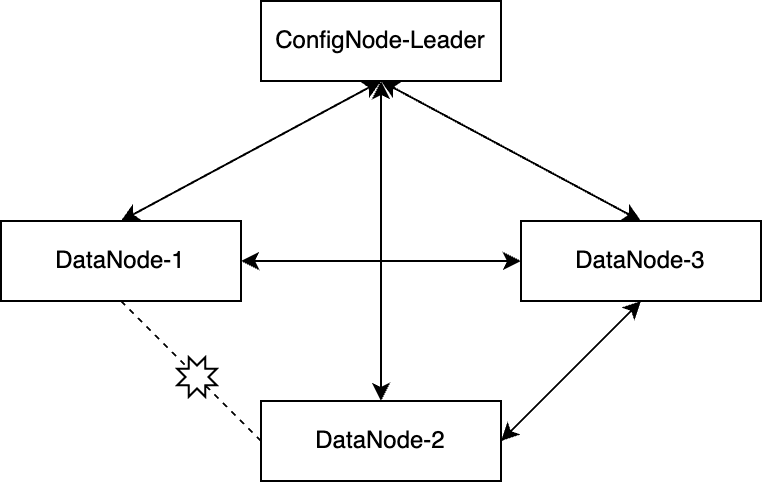
\includegraphics[width=0.7\linewidth]{c03-parition.png}
  \caption{系统非对称分区示意图}
  \label{fig:c03-partition}
\end{figure}

考虑图\ref{fig:c03-partition}所示的系统情况,集群由1个管理节点和3个数据节点组成,其中管理节点和所有三个数据节点都能正常连接交换情况,但是数据节点1和数据节点2之间的网络连接可能因为配置不当或者线缆断裂而出现非对称网络分区。这种非对称网络分区的问题不能被IoTDB已有的错误检测机制捕捉。这种未被检测到的非对称网络分区会极大地影响系统的可用性,可能造成的问题包括但不限于:

1. 影响共识模块的可用性保证。在RatisConsensus中,如果是两副本,并且两个副本分别处在非对称分区的两个节点数据节点1和数据节点2上,那么这个共识组在事实情况下处在不可用状态,需要进行相关的恢复策略。

2. 影响数据节点对客户端提供的服务保证。如果客户端需要将数据写入集群,且副本位于数据节点2上,那么客户端只能连接数据节点2直接写入或者通过数据节点3进行转发。如果客户端连接数据节点这次写入会在超时后失败,影响系统的高可用性保障。

3. 影响集群的查询能力。集群在查询调度的规划时,如果对网络可达性不了解,那么查询计划可能会错误的生成,导致这个查询计划最终失败。在章节\ref{sec:topology-query-plan}中对这一部分的错误有详细的说明。

\subsection{集群变更状态的不一致}

在分布式系统中,为应对业务负载变化、数据增长、节点故障或硬件升级等情况,系统需要具备弹性伸缩、负载均衡和故障恢复的能力。这些能力通常通过集群状态变更来实现,例如扩容/缩容,数据/副本迁移,副本数变更等。

这些变更操作都需要在集群中的多个节点之间进行协调和数据同步。在变更操作进行的过程中,系统会经历一个从旧状态到新状态的过渡阶段。在这个过渡阶段,由于信息传播的延迟或操作的异步性,集群中不同节点对整个系统状态(数据分片的位置、哪个副本是主副本等)的认知可能暂时不一致

严格来讲,集群变更的短暂不一致并非故障或错误,而是系统设计的有意为之。

根据CAP原理\cite{fox1999harvest},在一个分布式系统中,一致性(Consistency)、可用性(Availability)、分区容错性(Partition Tolerance)往往无法全部保证。在实际的系统中,分区问题无法避免,因此分区容错性必须保证。这导致一致性(Consistency)、可用性(Availability)只能二选一。

应用到IoTDB的集群变更场景来说,如果要保证集群变更期间的数据绝对一致性,那么必须暂停所有用户针对变更数据分区的写入操作,直至变更完成。
这种做法虽然保证了一致性,但却极大地牺牲系统的可用性,导致用户在一段时间内无法正常访问或操作数据,这跟本文的理念背道而驰。
因此,IoTDB在设计上允许变更期间的请求的正常执行,
通过额外的可用性方案在内部保证一致性。


\section{高可用和容错框架设计}

为应对上述提到的节点宕机、网络分区、磁盘空间不足等多种潜在故障,确保服务的持续可用和数据的可靠性,我们设计并实现了一个分层的高可用与容错框架,该框架的核心由故障检测、\failover 和故障恢复三部分组成,并依赖于管理节点、数据节点和客户端的协同工作。

\subsection{故障检测}

故障检测是整个高可用和容错框架的基础。其目标是快速、准确地发现集群中节点或网络链路的异常状态。快速检测能够缩短从故障发生到系统响应的时间,从而降低 RTO;准确检测能够避免误判,减少不必要的恢复或转移操作。

故障检测的基础是节点状态探测,主要通过节点周期性使用心跳对其他节点的存活状态探测来实现:

1.管理节点探测其他管理节点:管理节点 集群通过 Raft 共识协议内置的心跳机制相互探测,感知对等节点的存活,如果长时间未收到领导者的心跳就会触发新的选举。

2.管理节点探测所有数据节点:管理节点 作为集群元数据管理者,需要了解所有数据节点的健康状态以便进行负载均衡、数据迁移和故障转移决策。管理节点 会周期性地通过集群内部的RPC 调用向数据节点发送心跳请求,根据数据节点的响应来判断其是否存活和健康,以及节点上的资源情况、每一个共识组的情况。

3.数据节点探测所有其他的数据节点:数据节点会探知其他数据节点的状态,形成集群的拓扑。它们通过集群内部的RPC 调用来探测的拓扑状态,并将结果汇报给管理节点的领导者。

4.客户端探测数据节点:客户端通过尝试与数据节点建立和维持 TCP 连接,以及发送请求并等待响应来探测数据节点的可达性和可用性。连接建立失败、连接异常断开、或请求在合理时间内无响应都被客户端视为数据节点可能存在问题的信号。


有这些底层的心跳探测结果后,系统通过故障研判算法来判断一个节点是否确实处于故障状态。本文为IoTDB实现的研判算法包括:

1. 固定超时算法。如果在一个固定的时间内未收到心跳响应,则认为节点故障。优点是实现简单;缺点是无法适应变化的网络延迟,可能导致误判。

2. Phi Accrual 算法。 Phi Accrual是一种更自适应的故障检测算法,它不直接判断故障,而是计算一个节点的怀疑度。怀疑度基于心跳或探测消息的接收时间间隔,反应该节点可能发生故障的概率。当怀疑度超过预设的阈值时,系统就认为该节点“可能”发生故障。该算法的优点是能够根据历史网络延迟信息动态调整判断阈值,减少误判,更适合复杂网络环境;缺点是实现相对复杂。

3.基于TCP连接状态的算法。当集群管理节点与某个节点的 TCP 连接异常断开(如 RST 信号、连接超时)时,管理节点会立即判断该节点不可用。该方法的优点是快速且准确反映连接的即时状态。

通过以上多种探测机制和判断算法的结合使用,系统能够较全面、更为快速感知集群中出现的故障。


\subsection{\failover 和恢复}

\failover 是指在检测到某个节点或组件发生故障后,系统自动将受该故障影响的服务或数据访问无缝地切换到其他健康的、具有冗余能力的节点或副本上,以最小化对客户端的影响。该能力主要依赖共识模块的多副本能力,需要管理节点、数据节点和客户端客户端协同完成。

\failover 可以分解为以下三个阶段实现:

阶段一:请求规划阶段。在对读写请求形成分布式计划时,系统会根据管理节点提供的已知故障情况,智能地选择将请求发送到健康的副本所在的数据节点,从而避开已知故障或者不可达的节点。这是避开已知错误的主要手段。

阶段二:请求执行阶段。如果在尝试与某个副本通信时发生错误(例如,该副本恰好在规划阶段之后、执行阶段之前发生新的故障,或者存在短暂的网络抖动,导致通信失败),系统可以在同组的其他健康副本上进行重试,这一阶段的重试是为应对在请求执行过程中遇到的未知或临时的错误。这些错误可能是规划阶段未能及时感知的新故障,或者是特定连接上的瞬时网络问题。通过在多个副本上尝试执行,提高请求成功的概率,实现副本级别的故障转移能力,解决未知错误。

阶段三:请求重试阶段。如果经历规划阶段的初始路由选择和执行阶段的副本级重试后,客户端的请求仍然未能成功完成,客户端会进行兜底和重试。这一阶段是为整个客户端请求提供的最终容错保障。它处理由于客户端元数据严重过期、或者集群状态在短时间内发生剧烈变化导致前面阶段的重试都无效的情况。通过刷新元数据并重新尝试,客户端能处理更复杂的故障场景。

对于故障或落后的节点,当其重启和恢复时,共识模块会帮助其数据同步。共识模块会通过同步操作日志、同步WAL或者同步TsFile的方式让重启的节点赶上进度,增加集群的可用资源,保证集群的大多数副本在线。


\section{本章小结}

本章节对分布式系统的故障类型进行了总结,并分析概括几类通用的故障情况:进程宕机、磁盘空间不足、网络分区和集群变更不一致性。针对每类故障,本章探讨其成因、表现及其对分布式系统的具体影响。

接着,本章节提出Apache IoTDB 的高可用与容错框架,用于系统性地解决上述问题。该框架的核心由故障检测、\failover 和故障恢复,并依赖于管理节点、数据节点和客户端客户端的协同工作。